%           %experimenting with svn-multi

\svnkwsave{$RepoFile: siminos/froehlich/flow.tex $}
\svnidlong {$HeadURL$}
{$LastChangedDate$}
{$LastChangedRevision$} {$LastChangedBy$}
\svnid{$Id$}


\chapter{\CLf}
\label{chap:CLF}

\begin{quote}
{\bf Abstract:}
    {\color{red}
Stefan, write this: often! this might be the only part
of this text that most people glance at.
    }
\end{quote}

\section{Introduction}
\label{sect:intro}
     \Private{
\noindent{\bf Stefan -
Jun - Sep 2010}:\\
     }
This project first reproduces results reported by
Siminos\rf{SiminosThesis}, and then investigates various ways
of `quotienting' the \SOn{2} symmetry of \cLe, and reducing
the dynamics to symmetry 4-dimensional \reducedsp.
     \PC{
   When you write
   a project report or a research article, you always write abstract, introduction
   and conclusions first, and then keep rewriting them often.
   They are the most important parts of the text, as that is
   for most people only parts they will look at.
   }


The project consists of my notes and exercises.
    %
    \Private{ % subversion label pages
$\footnotemark\footnotetext{{\tt \svnkw{RepoFile}}, rev. \svnfilerev:
 last edit by \svnFullAuthor{\svnfileauthor},
 \svnfilemonth/\svnfileday/\svnfileyear}$
    } % end \Private{

The \cLe\ were introduced by Gibbon and McGuinness\rf{GibMcCLE82}
as a low-dimensional model of baroclinic instability in the
atmosphere. In the complex form, they are given by
\beq
\begin{split}
 \dot{x} &=-\sigma x+ \sigma y \\
 \dot{y} &=(r-z)x-a y \\
 \dot{z} &= \frac{1}{2}(x y^*+x^*y)-b z\,
 \label{eq:CLe}
\end{split}
\eeq
where $x,y$, $r=r_1+ i\,r_2$, $a=1+i\,e$ are complex and $z$,
$b$, $\sigma$ are real. Rewritten in terms of real variables
$x=x_1+ i\, x_2\,,\ y=y_1+i\, y_2$, \cLe\ are a 5-dimensional
first order ODE system\rf{SiminosThesis}
\beq
\begin{split}
	\dot{x}_1 &= -\sigma x_1 + \sigma y_1\\
	\dot{x}_2 &= -\sigma x_2 + \sigma y_2\\
	\dot{y}_1 &= (r_1-z) x_1 - r_2 x_2 -y_1-e y_2 \\
	\dot{y}_2 &= r_2 x_1 + (r_1-z) x_2 + e y_1- y_2\\
	\dot{z} &= -b z + x_1 y_1 + x_2 y_2\,.
	\label{eq:CLeR}
\end{split}
\eeq
In all numerical calculations that follow we shall set the
parameters to the Siminos values\rf{SiminosThesis},
\beq
r_1=28,\; b=\frac{8}{3},\;
\sigma=10,\; e=\frac{1}{10},\quad \mbox{and} \quad r_2=0
\,.
\ee{SiminosPrmts}

Here we are not interested in the physical applications of
these equations; rather, we study them as a simple example of
a dynamical system with continuous (but no discrete)
symmetries. Our goal is to find computationally
straightforward method of reducing the dynamics to a
lower-dimensional \statesp, where each group orbit of the
full system (\ie, set of translationally equivalent states)
is represented by a single point. If successful, the methods
that we develop might be applicable to very high-dimensional
flows, such as translationally equivariant fluid flows
bounded by pipes or planes\rf{GHCW07,GibsonMovies}.

\noindent {\bf Acknowledgments.}
This report is written in collaboration with
% E.~Siminos and
P.~Cvitanovi\'c.
S.F. work was supported by the National Science Foundation
grant DMR~0820054 and a Georgia Tech President's Undergraduate
Research Award.
P.C. thanks Glen Robinson Jr. for support.

\subsection{Visualizing \cLf}

In \refexer{exer:PlotCLf} we simulate \cLf\ in order to
visualize its long-time dynamics, as in
\reffig{fig:CLEx1x2z}. The dynamics is a big mess - the
trajectory seems to oscillate while drifting around $z$-axis.
Of most importance in \reffig{fig:CLEx1x2z}, is to notice
that the flow has a rotational symmetry about the $z$-axis.
Throughout the rest of the project we will try to find more
illuminating ways of understanding the dynamics of this flow
as well as ways of ``cleaning it up''--that is, removing this
symmetry and reducing the ODE system from five dimensions to
four.
    \PC{label axes, use legible fonts in all figures.}
    \PC{to Stefan: put all single figures into SFIG format, as
        \reffig{fig:CLEx1x2z}. If \reffig{fig:CLEx1x2z} was
        Rebecca's, replace it by your own figure.}
                                                    \exerbox{exer:PlotCLf}

%%%%%%%%%%%%%%%%%%%%%%%%%%%%%%%%%%%%%%%%%%%%%%%%%%
% computed by graphs.nb
\SFIG{CLEx1x2z}
{}{
A typical $\{x_1,x_2,z\}$ plot of the \cLf\ strange attractor,
with initial point
$(x_1, x_2, y_1, y_2, z) = (1, 0, 0, 1, 1)$.
    }{fig:CLEx1x2z}
%%%%%%%%%%%%%%%%%%%%%%%%%%%%%%%%%%%%%%%%%%%%%%%%%%


\section{Linear stability}
\label{sect:stability}
%\PC{Write up here the general text on stability, following \refref{DasBuch},
%\\
%\wwwcb{/chapters/stability.pdf}
%    }

When studying the trajectories of a flow, it is useful to
know how small neighborhoods of points are transported by the
flow. Understanding this gives us a better idea of how

Consider the displacement of an infinitesimally close
neighbor $x+\delta x$. Taylor expanding the flow equation
$\dot x = v(x)$ we find that
\beq
\dot x + \dot{\delta x}=v_i(x+\delta x) \approx v_i(x)+\Mvar \delta x
\eeq
where we shall refer to the matrix of velocity gradients
\beq
\Mvar_{ij}(x)=\frac{\partial v_i (x)}{\partial x_j}
\ee{SF:stabMat}
as the \stabmat.
In our first attempt to understand the dynamics of the flow,
we examine the \eqv\ of the system by finding this \stabmat\
$\Mvar$. For the \cLe\ it is the $[5\!\times\!5]$
matrix of velocity gradients,
                                                    \exerbox{exer:StabmatCLf}
\beq
  \Mvar =\left(\barr{ccccc}
    -\sigma    	& 0 		& \sigma & 0    &  0 \\
	0 	& -\sigma       & 0      & \sigma   &  0 \\
	r_1-z  &     -r_2      & -1     & -e & -x_1 \\
	r_2     & r_1-z       	& e  	& -1       & -x_2 \\
	y_1     & y_2           & x_1    & x_2      & -b
    \earr\right)
\eeq
As explained in ChaosBook.org\rf{DasBuch}, a \stabmat\
describes the instantaneous rate of shearing of the
infinitesimal neighborhood of $x(t)$ by the flow. That is, it
describes how quickly points initially very near to $x(t)$ will
diverge away from / converge to it in time. Matrix $\Mvar$ is an important
tool which we will use in what follows.

\subsection{\jacobianM}

We start by a discussion of the stability of \eqva\ and \po s,
and postpone the discussion of the stability of \reqva\ and \rpo s,
quintessentially continuous symmetry effects, to \refsect{SF:rpos}.

Consider the trajectory of a  neighbor infinitesimally close
to $\xInit$. Taylor expanding a finite time flow, we find that
\[
f^t(\xInit +\delta x) \approx f^t(\xInit)+\jMps^t(\xInit)\delta x,
\]
where
\beq
\jMps^t(x)_{ij}=\frac{\partial x_i(t)}{\partial x_j}
\ee{SF:jacMat}
 is
the \jacobianM. This means that up to the linear term the
neighborhood is transported by $\delta x(t)=\jMps^t(\xInit)\delta
\xInit$. This means that how nearby trajectories separate or
approach each other is dependent on the eigenvectors and
values of the \jacobianM.

The \jacobianM\ also maps the initial, Lagrangian coordinate
frame to the Eulerian coordinate at time $t$,
\beq
\velField{\ssp(t)}=\jMps^t(\xInit) \velField{\xInit}
\,,
\ee{JacobVeloc}
see \refexer{traLocEigFr}.
    \PC{remember to move \refexer{traLocEigFr}
    and its solution into ChaosBook. Currently it
    appears too early, search for ``traLocEigFr.''
    }

The methods of calculating the \jacobianM\ are discussed in ChaosBook.org\rf{DasBuch} where it is shown that the \jacobianM\ matrix is related to the stability matrix by $\frac{d}{dt} \jMps^t(x)=\Mvar (x) \jMps^t(x)$ or equivalently $\jMps^t(\xInit)= \texttt{T} e^{\int^t_0 d\tau \Mvar (x(\tau))}$, where \texttt{T} stands for a time-ordered product. When using a numerical routine to integrate the equations of motion, using a discrete approximation of either of these two formulas requires minimal additional programming effort.

% PC 13jul2010
\exercise{Transport of local eigenframes.}{     \label{traLocEigFr}
    \toCB
\noindent (a)
Derive \refeq{JacobVeloc}.
(b)
More generally, consider the
eigen\-vectors $\jEigvec[j]$ of $\jMps^t(\ssp)$
(sometimes referred to as `covariant Lyapunov vectors,'
or, for \po s, as `Floquet vectors')
\index{covariant Lyapunov vector}
\index{Lyapunov!covariant vector}
\beq
\jMps^t(\ssp)\, \jEigvec[j](\ssp(t))
   = \ExpaEig_{j}(t) \,\jEigvec[j] (\ssp(t))
\,,
\ee{finTimeEigs}
and show that a time $t'$ later they are transported into
eigenvectors $\jEigvec[j](\ssp(t+t'))$ of
$\jMps^{t+t'}(\ssp)$.
\authorPC{2010-07-12}
    }% end \exercise{Transport of local eigenframes.


\solution{traLocEigFr}{Transport of local eigenframes.}{
\noindent (a)
Consider two points that are an infinitesimal time apart along a trajectory:
$\delta \xInit
  = \flow{\timeStep}{\xInit}-\xInit \approx \velField{\xInit}\timeStep$.
As $\flow{t+\timeStep}{\xInit} =
\map^t \circ \flow{\timeStep}{\xInit}=\map^{\timeStep} \circ \flow{t}{\xInit}$,
we have
$\flow{\timeStep}{\map^t(\xInit)}=\flow{\timeStep}{\ssp(t)}
\approx x(t) + \velField{\ssp(t)} \timeStep$ and
$\flow{t}{\flow{\timeStep}{\xInit}}
=\flow{t}{\xInit+\velField{\xInit} \timeStep}
\approx \flow{t}{\xInit} + \jMps^t(\xInit) \velField{\xInit} \timeStep$.
Putting these two equations together we get the desired
\refeq{JacobVeloc}.

\noindent (b)
Predrag: I am not sure that this statement is correct, please
prove or disprove. Basically, check that \refeq{SF:transpEigPO}
is true for any orbit, not only \po s.

A tangent subspace $T\pS^{(i)}$ of the \statesp\ is said to be {\em covariant} if
\beq
T\pS^{(i)}(\ssp(t)) = \jMps^t(\xInit) T\pS^{(i)}(\xInit)
\ee{SF:covSubsp}
This definition also applies to covariant vectors, if $T\pS(i)$ is one-dimensional.
Covariant subspaces
are co-moving with the tangent flow.
\authorSF{2010-07-??}
    }% end

\subsection{\Eqva}

An \eqv\ $\EQV{}$ is a point $\ssp_{\EQV{}}$ for which the
velocity field of an ordinary differential equation
$\dot{\ssp} = v(\ssp)$ is zero, $v(\ssp_{\EQV{}})=0$. These
are points where the flow does not move, and if it reaches an
equilibrium, the flow remains there. For the \cLe\, the
origin $\EQV{0}=(0, 0, 0, 0, 0)$ is always an equilibrium
point, but there are two more families of equilibrium when
both $r_2 + e=0$ and $r_1>1$. If we could set on of these
{\em infinitely precisely} as the initial point of the flow,
instead of seeing the messiness of \reffig{fig:CLEx1x2z}, we
would stay at this single point for all times. In any
simulation, for unstable \reqv\ the (finite precision)
trajectory eventually leaves this point.
                                                    \exerbox{exer:EquiCLe}

% \subsection{Stability of \eqva}

At an equilibrium, the flow manages to stay at a single
point, but what if we start at points near the equilibrium? Will
they collapse into the equilibrium, or will they diverge away
from it? In order to answer this, we find and examine the
eigenvalues and eigenvectors of \Mvar\ evaluated at the
equilibrium $\EQV{0}$, the origin.
                                                    \exerbox{exer:EigenE0}
For the \cLe\, we find that the eigenvalues are
        \PC{ChaosBook convention is to order eigenvalues
        from most positive (unstable) to the most negative,
        that is why I renumbered them. Try to follow that
        everywhere. Replace complex eigenvectors by the real,
        imaginary parts, as that is what you actually use - I
        did this in \refeq{eigVecQ1}. I might have introduced
        errors in renumbering them, so trust your own
        computations, especially regarding the
        \reffig{fig:CLEE0} comments.
        }
\beq
\begin{split}
\lambda_{1,2} &=11.8277 \pm 0.062985 i\\
\lambda_{3,4} &=-22.8277 \pm 0.037015 i\\
\lambda_5 &=-2.66667\\
\end{split}
\eeq
with the associated eigenvectors
    \PC{\label{suspectEigVecs}is suspect:
    real, im parts seem interchanged in $e_1$?}
\bea
e_{1} &=& e_2^* =(0.001321+0.4581 i, 0.4581-0.001321 i, i, 1, 0)
\label{suspectEigVecs}\\
e_3 &=& e_4^* = (0.002249-0.7795 i, -0.7795-0.002249 i, 2.8421+i, 1, 0)
\continue
e_5 &=& (0, 0, 0, 0, 1)
\,.
\nnu
\eea
By examining the eigensystem, we can get a sense of what
happens to points near the equilibrium $\EQV{0}$. The
numerical values of the real parts of the eigenvalues
determine how quickly the flow will converge onto or diverge
away from the equilibrium. For a positive real part the flow
will diverge, and for a negative real part it will converge.
Complex eigenvalues also indicate that the motion will be
spiraling.

For the \cLe\ equilibrium $\EQV{0}$, the values of the
imaginary parts are orders of magnitude smaller than the real
parts, so that there will be very little spiraling. The large
values of the real parts tell us that the flow will
diverge/converge from the equilibrium very quickly.
                                                    \exerbox{exer:PlotEigenE0}

To illustrate this, we plot the eigenvectors (as real and
imaginary parts) and the flow at initial points very close to
$\EQV{0}$. The two real vectors (corresponding to a single
complex eigenvector) define the plane in which the flow will
spiral. We initiate the flow very close to $\EQV{0}$ at a
point along one of these vectors. In \reffig{fig:CLEE0},
we can see that for the vectors with a very small imaginary
part and a positive real part, the flow does not spiral
noticeably and that it diverges away from the equilibrium very
quickly.


\subsection{\Po s}{
\label{sect:SFpos}

We can extend this analysis of linear stability to not only
work for single points, but also allow us to study the
dynamics of the system near periodic orbits.

Let $p$ be a prime cycle, $\ssp \in M_p$ be any point on the
cycle, $\period{p}$ the period of the cycle and
$\jMps_p\left(\ssp\right) = \jMps^{\period{p}}(\ssp)$ be
the {\jacobianM} for a single transversal of the cycle.
The {\jacobianM} for the $r$th repeat of the cycle is then
$\jMps^{r
\period{p}}\left(\ssp\right)=\jMps^{\period{p}}\left(f^{\left(r-1\right)
\period{p}}\left(\ssp\right)\right) \cdots
\jMps^{\period{p}}\left(f^{\period{p}}\left(\ssp\right)\right)\jMps^{\period{p}}\left(\ssp\right)
=\jMps_p\left(\ssp\right)^r$
This means that it suffices to only look at prime cycles when
considering the {\jacobianMs} of periodic orbits.

Next consider the {\jacobianM} of a prime cycle $p$.
Using what we know from Jacobians,
$\delta \ssp \left(t+\period{p}\right)
=\jMps_p\left(\ssp\right)\delta \ssp\left(t\right)$
so after traveling once around the cycle, it contracts along
the directions of the Floquet vectors with Floquet
multipliers of magnitude less than 1 and expand in the
directions of Floquet vectors with Floquet multipliers of
magnitude greater than 1.

Now this only tells us the rate of contraction and expansion
as the cycle is traversed, starting at a point $\ssp$, it
would be nice to now how it behaves as it traverses every
part of the cycle.

The value of $\jMps_p\left(\ssp\right)$ depends on the point
on the periodic orbit chosen, but, as we shall show, the
Floquet multipliers are independent of this selection. To see
this, let $\ssp$ be any point on the cycle and
$\jEigvec[j]\left(\ssp\right)$ be a Floquet vector of
$\jMps_p\left(\ssp\right)$ with Floquet multiplier
$\ExpaEig_j$. Consider another
point  $\ssp'=f^t\left(\ssp\right)$, $ 0 < t < \period{p} $
on the periodic orbit. $\jMps^{\period{p} +t}=\jMps^{t+\period{p}}$,
{\jacobianMs} are multiplicative along the flow:
\bea
\jMps^{\period{p}+t}\left(\ssp\right)
&=&\jMps^{\period{p}}\left(f^t\left(\ssp\right)\right)\jMps^t\left(\ssp\right)
=\jMps_p\left(\ssp'\right)\jMps^t\left(\ssp\right)
\continue
\jMps^{t+\period{p}}\left(\ssp\right)
&=&\jMps^t\left(f^{\period{p}}\left(\ssp\right)\right)\jMps^{\period{p}}\left(\ssp\right)
=\jMps^t\left(\ssp\right)\jMps_p\left(\ssp\right)
\,,
\nnu
\eea
and
\bea
\jMps_p\left(\ssp'\right)\jMps^t\left(\ssp\right)\jEigvec[j]\left(\ssp\right)
&=&\jMps^t\left(\ssp\right)\jMps_p\left(\ssp\right)\jEigvec[j]\left(\ssp\right)
    \continue
&=&\jMps^t\left(\ssp\right)\left(\ExpaEig_j \jEigvec[j]\left(\ssp\right)\right)
=\ExpaEig_j \left(\jMps^t(\ssp) \jEigvec[j](\ssp)\right)
\continue
\jMps_p\left(\ssp'\right) \jEigvec[j]\left(\ssp'\right)
&=& \ExpaEig_j
\jEigvec[j]\left(\ssp'\right)
\,,
\label{SF:transpEigPO}
\eea
where
$\jEigvec[j]\left(\ssp'\right)
 = \jMps^t\left(\ssp\right)\jEigvec[j]\left(\ssp\right)$
 is the $\jMps_p$ eigenframe transported for time $t$
 along the $p$ orbit.
So $\ExpaEig_j$ is a Floquet multiplier for
$\jMps_p\left(\ssp'\right)$ too.

\section{Symmetries of dynamics}
\label{sect:SymmDyn}

         \Private{
\noindent{\bf Stefan -
Sep ?? 2010}:\\
\medskip\noindent
         }
In order to eventually remove the rotational symmetry in the
\cLf\, we need to show that the flow is rotationally
equivariant. By showing this, we will then be able to apply
algorithms to remove the symmetry. Rotational equivariance in
this situation will let us commute a rotation operator with
taking time derivatives.

We begin by defining the notion of `equivariance.'
A flow $\dot{x}= \vel(x)$ is \emph{equivariant} under an operation $\LieEl$ when
\beq
\LieEl \, \vel(x)=v(\LieEl \, x)
\,.
\ee{eq:FiniteRot}
This means that if $f(x)$ is a solution to the dynamical
equations, then so is $\LieEl\,f(x)$.

In many flows (the \cLe\ are a particularly simple example),
the equivariant operations
will form a Lie group that can be used to reduce the
dynamics.

\subsection{Lie groups}

A theory of Lie groups is a vast subject. This report follows the notational conventions of ChaosBook.org\rf{DasBuch}. We found Roger Penrose\rf{Penr04} introduction to the subject both enjoyable and understandable.
    \PC{to PC - remember to copy \refref{Penr04} to ChaosBook.org.}

A Lie group is a group which (1) is a differential manifold
and (2) the composition map $G \times G \rightarrow G : (g,h)
\rightarrow g h^{-1}$ is $\mathbb{C}^\infty$.
    \PC{Stefan, this looks like a rather unenlightening definition.
        Can you make up a more useful one?}
As its representations are everywhere differentiable, an element of a compact Lie group can be parameterized in exponential form.
    \PC{Stefan wrote: ``By assumption the Lie group of symmetries is compact and connected;'' then ``we don't need connected, we just need a representation of the group elements that is differentiable, and there is one for $\On{n}$. For a group like $\On{n}$ you have two connected components, proof presumably still works? {\bf PC}: Agreed. 'Compact' is not needed, either}
For example,
an element of a compact Lie group that is continuously
connected to the identity can be expressed as
\beq
\LieEl(\gSpace)=e^{{\gSpace} \cdot \Lg }
\,,
\ee{FiniteRot}
where $\gSpace \cdot \Lg$ is a \emph{Lie algebra} element,
and the $\gSpace_a$ are the parameters of the transformation.
    \PC{need to generalize to groups like \On{n}}
                                                    \exerbox{exer:FinRot2d}
%
A rotation by an infinitesimal amount, $|\delta \gSpace| \ll
1$, can be expressed as
\[
\LieEl(\delta \gSpace) \simeq 1 + \delta \gSpace \cdot \Lg
\,,
\]
where the $\Lg_a$ are a set of N linearly independent
$[d\times d]$ antihermitian matrices acting linearly on the
{\statesp}. They are called the \emph{generators} of
infinitesimal transformations.
To see why, define the group action tangent at $\ssp$,
\beq
 \groupTan_{a}(\ssp) = \Lg _{a} \ssp
    \,,\qquad
 a=1,2,\cdots,N,
\ee{PC:groupTan}
and consider a transformation induced by an infinitesimal
time-dependent variation of group `phases'
$\delta \gSpace_a = \timeStep \, \dot{\gSpace_a}$,
\[
\delta \ssp = \timeStep \dot{\gSpace} \cdot \groupTan(\ssp)
\,.
\]
So $\dot{\gSpace} \cdot \groupTan(\ssp)$ is the velocity
of the flow along the group orbit of \ssp.
We shall use $\groupTan_a(\sspRed)$ notation (rather than
$\Lg_{a}\sspRed$) to emphasize that the group action
induces a \emph{tangent field} at $\sspRed$.

The statement of equivariance
$
\dot{x}=\LieEl^{-1} \vel(\LieEl x)
$
for infinitesimal rotations is
\[
\dot{x}=(1-\gSpace \cdot \Lg ) \vel(x+\gSpace \cdot \Lg  x)
       =\vel(x)-\gSpace \cdot \left(
            \Lg \vel(x) - \frac{d\vel}{dx} \Lg x
                     \right)
\,.
\]
We can now state the {\em infinitesimal
rotations} version of the equivariance condition
\refeq{eq:FiniteRot} as:
\beq
0 = - \groupTan_{a}(\vel)+\Mvar \groupTan_{a}(\ssp)
\,,
\label{eq:InfnmslRot}
\eeq
where $\Mvar$ is the \stabmat\ \refeq{SF:stabMat}.
% \refeq{5x5stabMat}.
    \PC{Stefan, you might want to learn about Jacobi derivatives,
        explain this statement geometrically}

We have used both this infinitesimal rotation condition and
the finite angle rotation condition \refeq{eq:FiniteRot}, to
verify that the \cLe\ are rotationally equivariant.
    \PC{Stefan, have you done this? Yes or no.}
                                                    \exerbox{exer:InfinRotInvari}
                                                    \exerbox{exer:FinRotInvarCmplx}
                                                    \exerbox{exer:FinRotInvari}


%\paragraph{Definition:           Fixed-point subspace}
\begin{definition}
\label{def:centralizer}
\index{slice}
\textbf{Fixed-point subspace.}
\index{centralizer}\index{fixed-point subspace}
\index{G-fixed@\Group-fixed}\index{fixed point!under \Group}
$\pS_H$ of a subgroup or a `centralizer' $H \subset \Group$,
$\Group$ a symmetry of dynamics, is the set of all \statesp\
points left \emph{$H$-fixed}, \emph{point-wise} invariant
under subgroup action
\beq
\pS_H = \Fix{H} =
   \{ \ssp \in \pS : {h} \, \ssp = \ssp \mbox{ for all } h \in H \}
\,.
\ee{dscr:FPsubsp}
% \paragraph{Definition:         Invariants.}
\index{invariant!points}
Points in the \emph{fixed-point subspace}  $\pS_\Group$ are fixed
points of the full group action. They are called \emph{invariant
points},
	\index{invariant!points}
\beq
\pS_\Group = \Fix{\Group} =
   \{ \ssp \in \pS : {g} \, \ssp = \ssp \mbox{ for all } g \in \Group \}
\,.
\ee{dscr:InvPoints}
\end{definition}
		%
		                                                  \toCB

%
%%%%%%%%%%%%%%%%%%%%%%%%%%%%%%%%%%%%%%%%%%%%%%%%%
\example{\SOn{2} irreducible representations:}{
    \label{exam:SO2irrepst}
    \index{SO(2)@\SOn{2}!irreducible representation}
%DB% (continued from \refexam{exmp:contSO2rot})~~
Expand a smooth periodic function $u(\gSpace + 2\pi) =
u(\gSpace)$ as a Fourier series
\beq
u(\gSpace) = \frac{a_0}{2} + \sum_{m=1}^\infty \left(
a_m \cos m \gSpace + b_m \sin m \gSpace
                               \right)
\,.
\ee{FourierExp}
The matrix representation of the \SOn{2}\ action
%DB% \refeq{SO2LieFunct}
on the $m$th Fourier coefficient pair
$(a_m,b_m)$ is                                      \toCB
\beq
\LieEl^{(m)}(\gSpace') \,=\,  \left(\barr{cc}
 ~\cos m \gSpace'  & \sin m \gSpace' \\
 -\sin m \gSpace'  & \cos m \gSpace'
    \earr\right)
= \cos m \gSpace' \id^{(m)}
  + \sin m \gSpace'\, \frac{1}{m} \Lg^{(m)}
\,,
\ee{SO2irrepAlg-m}
with the Lie group generator
    \index{generator!anti-hermitian}
    \index{anti-hermitian!generator}
\beq
 \Lg^{(m)} \,=\,   \left(\barr{cc}
    0  &  m  \\
   -m  &  0
    \earr\right)
\,.
\ee{SO2irrepAlg-Lg}
$\id^{(m)}$ is the identity, $\Lg^{(m)}$ is the Lie
algebra generator on the $m$-irreducible
subspace, 0 elsewhere.
The \SOn{2}\ group tangent $\groupTan(u)$
%DB% \refeq{GroupTangField}
to \statesp\ point $u(\gSpace)$ is the sum over invariant subspace
contributions                           \toCB
\beq
 \groupTan(u) = \sum_{m=1}^\infty \groupTan^{(m)}(u)
    \,,\qquad
 \groupTan^{(m)}(u)
\,=\, m \,\left(\barr{c}
   ~b_m  \\
   -a_m
    \earr\right)
\,.
\ee{u:x:tang}
The $L^2$ norm of $\groupTan(u)$ is weighted by
the \SOn{2}\ quadratic Casimir \refeq{QuadCasimir},
$C_2^{(m)} = m^2$,
\beq
\oint \frac{d\gSpace}{2\pi}
     \, (\Lg u(\gSpace))^T \Lg u(2\pi-\gSpace)
= \sum_{m=1}^\infty m^2 \left(a_m^2 + b_m^2\right)
\,,
\ee{tangL2norm}
and converges only for sufficiently smooth $u(\gSpace)$. What
does that mean?
%DB% We saw in \refeq{RPOtrans_gen} that
$\Lg$ generates translations, and by \refeq{SO2irrepAlg-Lg} the
velocity of the $m$th Fourier mode is $m$ times higher than for the $m=1$
component. If $| u^{(m)}| $ does not fall off faster the $1/m$,
the action of \SOn{2}\ is overwhelmed by the high Fourier modes.
    } % end \example{\SOn{2} irreps
%%%%%%%%%%%%%%%%%%%%%%%%%%%%%%%%%%%%%%%%%%%%%%%%%
%

%
%%%%%%%%%%%%%%%%%%%%%%%%%%%%%%%%%%%%%%%%%%%%%%%%%
\example{\SOn{2} rotations for \cLe:}{\label{exam:FinRot}
    \index{SO(2)@\SOn{2}}
The \SOn{2} symmetry group of \cLe\ acts on the
5-dim\-ens\-ion\-al space \refeq{eq:CLeR}
by a finite angle \SOn{2} rotation:
\index{generator!anti-hermitian}
\index{anti-hermitian!generator}
\beq
\LieEl(\gSpace) \,=\,  \left(\barr{ccccc}
  \cos \gSpace  & \sin \gSpace  & 0 & 0 & 0 \\
 -\sin \gSpace  & \cos \gSpace  & 0 & 0 & 0 \\
 0 & 0 &  \cos \gSpace & \sin \gSpace   & 0 \\
 0 & 0 & -\sin \gSpace & \cos \gSpace   & 0 \\
 0 & 0 & 0             & 0              & 1
    \earr\right)
\,.
\ee{CLfRots}
The corresponding Lie algebra generator is
    \PC{is the sign standard?}
\beq
 \Lg \,=\,   \left(\barr{ccccc}
    0  &  1 & 0  &  0 & 0  \\
   -1  &  0 & 0  &  0 & 0 \\
    0  &  0 & 0  &  1 & 0  \\
    0  &  0 &-1  &  0 & 0 \\
    0  &  0 & 0  &  0 & 0
    \earr\right)
\,.
\ee{CLfLieGen}
%From \refeq{SO2irrepAlg-m} we see that
The action of \SOn{2}\ on the \cLe\ \statesp\ thus decomposes into $m=0$ \Group-invariant subspace ($z$-axis) and  $m=1$ subspace with multiplicity 2.

The generator $\Lg$ is indeed anti-hermitian,
$\Lg^\dagger = - \Lg$, and the group is compact, its
elements parametrized by $\gSpace \mbox{ mod } 2\pi$. Locally, at
$\ssp \in \pS$, the infinitesimal action of the group is
given by the group tangent field $\groupTan(\ssp) = \Lg \ssp
= (x_2,-x_1,y_2,-y_1,0)$. In other words, the flow induced by
the group action is normal to the radial direction in the
$(x_1,x_2)$ and $(y_1,y_2)$ planes, while the $z$-axis is left
invariant.
    } % end \example{Finite angle \SOn{2} rotations:}{
%%%%%%%%%%%%%%%%%%%%%%%%%%%%%%%%%%%%%%%%%%%%%%%%%
%

\subsection{Inner products}
\label{def:innerProduct}
\index{slice}

As we shall use here several inner products:
over group manifolds, over real and complex finite-dimensional coordinates, and over function spaces, it is convenient to introduce a compact notation that subsumes them all as special cases.
    \PC{We need to define these properly. When we get to fluids, it's not trivial - we will use `energy norm.' }

Here the dot product $\gSpace \cdot \Lg$ shall refer to the sum over
the Lie algebra generators of an $N$-dimensional Lie group \Group,
\beq
\gSpace \cdot \Lg = \sum_{a=1}^N \gSpace_a \Lg_a
%    \,,\qquad a = 1,2,\cdots,N
\,.
\ee{dotGroup}
The inner product of two \statesp\ vectors $x, y \in \pS$ will be denoted by $\dotProd{x}{y}$. If the \statesp\ is of a finite dimension $d$ and real, the inner product is the Euclidian product of two vectors $x,y$,
\beq
\dotProd{x}{y} = \sum_i^d {x}_i y_i
    \,,\qquad \pS \subset \reals
\,.
\ee{innerR}
If the \statesp\ is finite dimensional and complex,
\beq
\dotProd{x}{y} = \sum_i^d \dual{x}_i y_i
    \,,\qquad \pS \subset \complex
\,,
\ee{innerC}
where $\dual{x}$ is the complex conjugate transpose of vector $x$, or, more generally, the hermitian conjugate $\dual{M}$ of matrix $M$. A matrix $M$ acts as
    \PC{This should probably be extended to non-selfadjoint
        actions, explain the adjoint {\jacobianM} $\dual{\jMps}$.}
\beq
\dotProd{x}{M\,y} =
  \dotProd{\dual{M}\,x}{y}
\,.
\ee{adjointG}
% where $\dual{M}$ is the hermitian conjugate of $M$.
If the \statesp\ is a normed function space (Banach, Hilbert, Sobolev, ...),
the inner product is given by the integral
\beq
\dotProd{g}{f} = \int dx \, \dual{g}(x) f(x)
\,.
\ee{innerL2}
The associated $L^2$ norm is
$|\ssp|^2 = \dotProd{\ssp}{\ssp} \neq 0$, unless $\ssp = 0$.

In computations the functions are expressed in terms of
complete orthonormal basis sets $\{u_n\}$,
\bea
f(x) &=& \sum_{n=0}^{\infty} a_n u_n(x)
    \continue
\dotProd{u_n}{u_m} &=& \delta_{nm}
\,.
\label{basisL2}
\eea
Unitary and orthogonal groups (as well as their subgroups) are
defined as groups that preserve these `length' norms,
$\dotProd{\LieEl x}{\LieEl x} =  \dotProd{x}{x}$, and
infinitesimally their generators induce no change in the norm,
\[
\dotProd{\dual{\Lg}_a\ssp}{\ssp}
  +\dotProd{\ssp}{\Lg_a\ssp} =0
\,,
\]
hence the Lie algebra generators
$\Lg$ are antisymmetric for orthogonal (sub)groups,
and antihermitian for unitary ones,
\beq
\dual{\Lg} = - \Lg
\,.
\ee{antiHerm}
This antisymmetry of generators
implies that the action of the group on vector $\ssp$ is
locally normal to it,
\beq
\dotProd{\groupTan_{a}(\ssp)}{\ssp} =0
\,.
\ee{TtimesX}

A group tangent \refeq{PC:groupTan} is a vector both in the group
tangent space and in the \statesp.
We shall indicate by $\dotProd{\groupTan_{a}(x)}{\groupTan_{b}(y)}$  the sum over \statesp\ inner product only, and by
\beq
\dotProd{\groupTan(x)}{\groupTan(y)} =
    \sum_{a=1}^N \dotProd{\groupTan_{a}(x)}{\groupTan_{a}(y)} =
  \dotProd{x}{\dual{\Lg} \cdot {\Lg}\,y}
\ee{innerGdot}
the sum over both group and spatial dimensions.

Any representation of a compact group $\Group$ is fully
reducible, and for a Lie group
the invariant tensors constructed by contractions
of $\Lg_a$ are useful for identifying irreducible
representations. The simplest such invariant is
\beq
\dual{\Lg} \cdot \Lg = \sum_\alpha C_2^{(\alpha)} \, \id^{(\alpha)}
\,,
\ee{QuadCasimir}
where $C_2^{(\alpha)}$ is the quadratic Casimir for
irreducible representation labeled $\alpha$, and
$\id^{(\alpha)}$ is the identity on the $\alpha$-irreducible
subspace, 0 elsewhere. $ C_2^{(\alpha)} =0$ if $\alpha$
is an invariant subspace.
The dot product of two tangent fields
\refeq{innerGdot} is thus a sum of inner products
weighted by Casimirs,
\beq
\dotProd{\groupTan(x)}{\groupTan(y)}
   = \sum_\alpha C_2^{(\alpha)} \dual{x}_i\, \delta_{ij}^{(\alpha)} y_j
\,.
\ee{dotProd}
For compact groups $C_2^{(\alpha)}$ are strictly nonnegative by
the antihermiticity \refeq{antiHerm} of Lie algebra generators.



\section{\Reducedsp}
\label{sect:reducedStateSp}

    \PC{Stefan explain the general concept of symmetry reduction first}
One of our goals of this project is to reduce the \statesp\ of the \cLe\ from five to four dimensions. We propose to accomplish this by the `{\mslices}.'

\subsection{\Mslices, finite time steps}
\label{sect:MovFrame}

     \Private{
\noindent{\bf Predrag -
July 19, Aug 12 2009; Sep 19 2010}
    }

Here we describe symmetry reduction by the
{\em {\mslices}} of
Cartan\rf{CartanMF,FelsOlver98,FelsOlver99,OlverInv}.
                                                \exerbox{exer:SO2cSect}
                                                \exerbox{exer:mslicesInv}
Split up the integration of an $\Group$-equivariant ODE into
a sequence of short time steps, each followed by a group action
such that the next segment initial point is in the point
$\sspRed \in$ {\slice}, a $(d\!-\!1)$-dimensional hyperplane
normal to the group rotation tangent $\sliceTan{}$ at point
$\slicep$:
    \PC{Stefan, rewrite the whole text in terms of
        $\dotProd{.}{.}$.}
\[ %beq
\dotProd{\sspRed - \slicep}{\sliceTan{a}}=0
    \,,\qquad
\sliceTan{a} = \Lg_a \slicep
\,.
\] %ee{PCsectQ}
For any $\ssp$, the slice condition $\sspRed =
\LieEl(\gSpace)\ssp$ determines the group
action $\LieEl(\gSpace)$ that brings $ \ssp$ into the \slice.
Such a map from a point in space to the group action is called a
\emph{moving frame} in the formulation of Fels and
Olver\rf{FelsOlver98,FelsOlver99,OlverInv}.

\begin{definition}
\label{def:slice}
\index{slice}
\textbf{\Slice}:
Pick a non-zero \emph{slice-fixing point} $\slicep \in \pS$.
We call the $(d\!-\!N)$-dimensional hyperplane $\sspRed \in \pSRed$
a \emph{\slice}, where
\(
\dotProd{\sspRed - \slicep}{\sliceTan{a}}=0
\) %ee{PCsectQ1}
is normal to all group tangents $ \sliceTan{a}= \Lg_a \slicep$ at $\slicep$. The {slice-fixing point} should lie outside the invariant subspace $\pS_\Group = \Fix{\Group}$ or any of the invariant subspaces $\pS_H$ defined in \refeq{dscr:FPsubsp}. Were \slicep\ invariant under the group, then $\sliceTan{a}=0$ and the ``\slice'' so defined would be the entire space.
    \PC{Extend this claim to the invariant subspaces as well}
    \PC{In constructing his return map, Lorenz, I think,
    used projections on the invariant axes $z$ and $\dot{z}$.
    Is that not a \slice? Rethink}

As $ \dotProd{\slicep}{\sliceTan{a}}=\dotProd{\slicep}{\Lg_a \slicep} =0 $ by \refeq{antiHerm} the antihermiticity of \Lg, the condition that a point \sspRed\ lies in the \slice\ \pSRed\ is
\beq
\dotProd{\sspRed}{\sliceTan{a}}=0
    \,,\qquad
\sliceTan{a} = \Lg_a \slicep
\,.
\ee{PCsectQ1}
\end{definition}
Note: while in general a {\slice} need not be a hyperplane,
we find the linear slice condition \refeq{PCsectQ1} easiest to implement.
For linear case, the same slice is fixed by any
point on the ray $const\; \slicep$ through the point \slicep.

\example{\CLe\ rotation angle.}{\label{exam:CLErotAngle}
To show how the rotation into the \slice\ is computed, consider first the \cLe. There is only one infinitesimal generator for the \SOn{2} symmetry group, so the \reducedsp\ trajectory is given by $\sspRed=\LieEl(\gSpace) \ssp$ where $\gSpace$ is such that $\dotProd{\sspRed}{\sliceTan{}}=0$. Substituting the \SOn{2}\ Lie algebra generator \refeq{CLfLieGen} and  a finite angle \SOn{2} rotation \refeq{CLfRots} acting on a 5-dim\-ens\-ion\-al space \refeq{eq:CLeR} into the slice condition \refeq{PCsectQ1} yields the explicit formula for $\gSpace$:
\beq
    \dotProd{\ssp}{\Lg \ssp'}\cos\gSpace+\dotProd{\Lg\ssp}{\Lg \ssp'} \sin\gSpace=0
\ee{SL:CLEsliceRot}
\[
     \tan\gSpace= - \frac{\dotProd{\ssp}{\Lg \ssp'}}
                      {\dotProd{\Lg\ssp}{\Lg \ssp'}}
\]
\[
    (x_1 x_2'-x_2 x_1'+y_1 y_2' -y_2 y_1')\cos\gSpace
    + (x_1 x'_1+x_2 x'_2+y_1 y'_1+y_2 y'_2)\sin\gSpace
=0
\,.
\]
    \PC{Stefan, I think you have to explain that, just as in the
    case of Poincar\'e sections, one keeps track of only oriented
    crossings, \ie, a circle has only on section in a \slice,
    not two. That should give you a precise $\pi$ rotation rule
    for singularity crossing.}
Note that if \gSpace\ is a solution, so is $\gSpace+\pi$.
This formula is particularly simple, as in this example the group
acts only through $m=0$ and $m=1$ representations; in general
the `phases' $\gSpace_a$ have to be computed numerically.

    }%end \example{\CLe\ rotation angle

[...]
                                                    \exerbox{exer:PCsectionCLe}
                                                    \exerbox{exer:SO2rotAngle}

%%%%%%%%%%%%%%%%%%%%%%%%%%%%%%%%%%%%%%%%%%%%%%%%%%
% computed by PCunrot.nb
\SFIG{ProblemsPill} %PCunrot}
{}{
{\Mslices}, finite time steps version: a
trajectory started on the \slice, with $\ssp_1^{(0)}
=0$, evolves for a finite time to a \statesp\ point with a
non-zero $\hat{\ssp}_1^{(1)}$. The {\em entire} \statesp\ is then
rotated (the `frame is moved') so that the equivalent point
on the circle lies on the \slice, $\ssp_1^{(1)} =0$.
Thus after every finite time step followed by a rotation the
trajectory returns to the 4$\dmn$ $\ssp_1 =0$
\reducedsp.
}
{fig:PCunrot}
%%%%%%%%%%%%%%%%%%%%%%%%%%%%%%%%%%%%%%%%%%%%%%%%%%

\refFig{fig:PCunrot} illustrates the {\mslices},
finite time version.
    \PC{Draw your own \refFig{fig:PCunrot}
        - need to draw a longer segment of the initial trajectory,
        to make it clearer that the whole segment is rotated.
       }

%
%%%%%%%%%%%%%%%%%%%%%%%%%%%%%%%%%%%%%%%%%%%%%%%%%
\exercise{\SOn{2}  rotation angle:}{\label{exer:SO2rotAngle}
Continue the discussion of \refexam{exam:SO2irrepst} and write down the formula for $\gSpace$ for a Fourier expansion of a periodic function. Show that now the \slice\ condition is a polynomial in $\cos\gSpace$, $\sin\gSpace$, and that, depending on the magnitudes of the Fourier series terms, the group orbit may traverse a slice arbitrarily many times.
    \PC{is it still true that the rotation is by $\pi$?}
    } %end \SOn{2}  rotation angle.

\exercise{Determination of group invariants by the {\mslices}:
    }{ \label{exer:mslicesInv}
Show that the $d-N$ \reducedsp\ coordinates determined by the {\mslices} are independent group invariants, and that the {\mslices} allows the determination of (in general non-polynomial) invariants of the group action by a simple  algorithm that works well in high-dimensional \statesp s.
    }

\solution{exer:mslicesInv}
{Determination of group invariants by the {\mslices}:}{
(To be written by Stefan: read and understand relevant parts of Fels and
Olver\rf{FelsOlver98,FelsOlver99,OlverInv}, Siminos\rf{SiminosThesis})
    }


\subsection{How good is your \slice?}
\label{sect:slices}

    \PC{this is a rewrite in progress of \refsect{sect:raw}}
For the \mslices\ to be operationally useful, we have to
(1) show that the given \slice\
cuts the group orbit of every point in the full \statesp,
(2) show how to continue an orbit through \slice\ discontinuities,
and
(3) find a criterion to pick a single \po\ amongst the {\reducedsp} \po s
arising from multiple traversal of a slice by a single  full space
\rpo\ES{If (1) is fullfiled then why do we need to worry about (2)? Or, what
do we mean by discontinuities?}.

We first show that \slice\ \refeq{PCsectQ1} intersects all group orbits in $\pS$.
Let $\ssp \in \pS$ be a point in the \statesp, and a group element represented  by $\LieEl=e^{\gSpace \cdot \Lg}$, as in \refeq{FiniteRot}.
    \PC{this looks like a repeat of what is to come, dropped: `` We want to show that there is a point on the group orbit of $\ssp$ which lies in \pSRed, \ie\ there exists a group element $\LieEl=e^{\gSpace \cdot \Lg}$, $\sspRed= \LieEl \ssp \in \pSRed$ such that $\dotProd{\LieEl \ssp}{\sliceTan{a}}=0$ for all $a$.
    ''}

Consider $f(\gSpace)=\dotProd{e^{\gSpace \cdot \Lg} \ssp}{\slicep}$, the projection of the group orbit of $\ssp$
onto the slice-fixing ray through \slicep.
\ES{} $f$ is a continuous and differentiable function of \gSpace. If $\ssp$ is invariant, its group orbit is itself, and $f(\gSpace)$ takes a constant value.

If $\gSpace_E$ is an extremum of $f$ then all of the first order partial derivatives of $f$ vanish at $\gSpace_E$, $\frac{\partial f(\gSpace_E)}{\partial \gSpace_a} =\dotProd{\Lg_a e^{\gSpace_E \cdot \Lg} \ssp}{\slicep}=0$. $\Lg_a$ is antihermitian, so
$0=\dotProd{\Lg_a e^{\gSpace_E \cdot \Lg}\ssp}{\slicep}
= - \dotProd{\LieEl_E \ssp}{\Lg_a  \slicep}$,
and
\[
\dotProd{\LieEl_E \ssp}{\sliceTan{a}} =0
\,.
\]
We therefore have that $\sspRed= \LieEl_E \ssp$ is normal to all the group tangents of $\ssp$ so it is in \pSRed. This means that the slice condition is satisfied by $\sspRed_E = \LieEl_E \ssp$ corresponding to an extremum of the $f$, and thus $\sspRed_E$ is in the slice. All that is left to do then is to show that $f$ has extrema. But as the group is compact, the group orbit of every point in \pS\ is compact, so its projection on the slice-point $\slicep$ has at least two extremal points, and thus every group orbit intersects the \slice. For example, group orbits of \SOn{2}\ are topologically circles, and their projections have maxima, minima and inflection points as extrema.
    \PC{
    Stefan, if I have removed some essential part of your proof, please restore it.
    The narrative continues in \refsect{sect:sliceSing}.
    }


\subsection{\Mslices, differential formulation}
\label{sect:MovFrameODE}


\begin{bartlett}
I made a wrong mistake.
\bauthor{Yogi Berra}
\end{bartlett}


                                                    \exerbox{exer:CLEsmall-x1x2}
                                                    \exerbox{exer:csectionCLeODE}
                                                    \exerbox{exer:csectionPhase}
Infinitesimal time version of the moving frames symmetry
reduction is attained by taking small time steps in
\reffig{fig:PCunrot} and dropping the higher order terms, as
in \refsect{sect:SymmDyn}.

Let $\sliceTan{}$ be a vector normal to the plane of the slice. Then the dynamics within the slice are given by
\bea
\dot{\gSpace_a}(\sspRed) &=& \frac{\dotProd{\vel(\sspRed)}{\sliceTan{a}}}
               {\dotProd{\groupTan(\sspRed)}{\sliceTan{}}}
\continue
\velRed(\sspRed) &=& \vel(\sspRed)
   -\dot{\gSpace}(\sspRed) \cdot \groupTan(\sspRed)
\label{SF:sliceEas}
\eea
where $\velRed(\sspRed)$ is the velocity in the slice.


%%%%%%%%%%%%%%%%%%%%%%%%%%%%%%%%%%%%%%%%%%%%%%%%%%
% File: infMF.xfig
\SFIG{ProblemsPill} %infMF}
{}{
Method of moving frames, infinitesimal formulation.
}
{fig:infMF}
%%%%%%%%%%%%%%%%%%%%%%%%%%%%%%%%%%%%%%%%%%%%%%%%%%

    \PC{Draw your own \reffig{fig:infMF}.
        }
                                                        \exerbox{exer:csectionReduced}
    \PC{
A more elegant derivation is given in
\refrefs{rowley_reconstruction_2000,rowley_reduction_2003}.
    }


%
%%%%%%%%%%%%%%%%%%%%%%%%%%%%%%%%%%%%%%%%%%%%%%%%%%%%%%%%%%%%%%%%%%
% CLEpcSect.png computed by  CLEfinal.nb (repo: vaggelis)
% CLEpcSect2.png computed by CLEfinal.nb (repo: vaggelis)
\begin{figure}[ht]
\begin{center}
(a) % 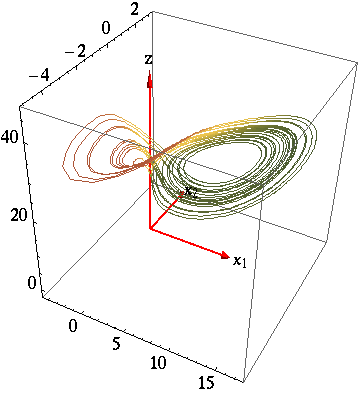
\includegraphics[width=0.40\textwidth]{CLEpcSect}
(b) %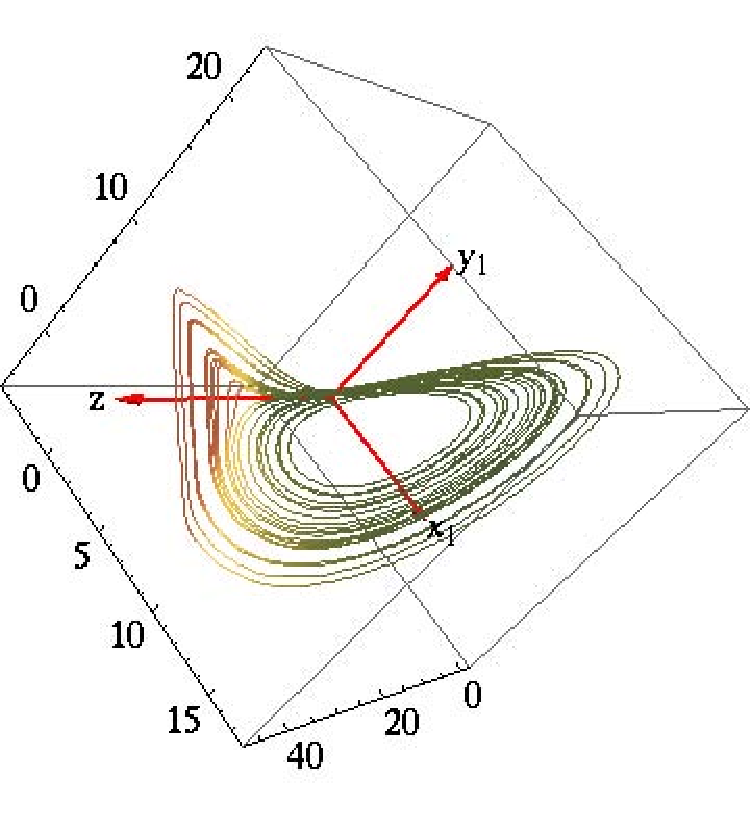
\includegraphics[width=0.43\textwidth]{CLEpcSect2}
\end{center}
\caption{
Method of moving frames, \slice\ fixed by a point on an
\reqv\ group orbit, $\sspRed = \ssp_{\REQB{}1}$. The strange
attractor of \reffig{fig:CLEx1x2z} in the \reducedsp\
of \refeq{EqMotionMovFramePC}:
(a) $\{x_1,x_2,z\}$ projection,
(b) $\{x_1,y_1,z\}$ projection.
Color-coding indicates $(\hat{\ssp} \cdot \hat{\sspRed})_4$
where $\hat{.}$ stands for unit vector, with green indicating values
of the inner product close to $1$ and brown indicating values
close to $0$.
    }
\label{fig:CLEpcSect}
\end{figure}
%%%%%%%%%%%%%%%%%%%%%%%%%%%%%%%%%%%%%%%%%%%%%%%%%%%%%%%%%%%%%%%%
%
A long time trajectory of \refeq{EqMotionMovFramePC} with
$x^*$ on the \reqv\ \REQB{1} group orbit is shown in
\reffig{fig:CLEpcSect}.
                                                        \exerbox{exer:PCsectionCLe}
    \PC{draw your own \reffig{fig:CLEpcSect}:\\
        * Mark $\ssp_{\REQB{}1}$ \\
        * Draw stable eigenvector of $\ssp_{\REQB{}1}$\\
        * State value of $\ssp_{\REQB{}1}$ somewhere
        }


%%%%%%%%%%%%%%%%%%%%%%%%%%%%%%%%%%%%%%%%%%%%%%%%%%
% computed by PCunrot.nb
\SFIG{ProblemsPill} %PCunrot1}
{}{
Method of moving frames, continuous time version, for the
$\slicep=(0,1,0,0)$,
$x_1=0,\;x_2>0$, \slice. The strange attractor of
\reffig{fig:CLEx1x2z} in the \reducedsp,
$\{x_2,y_2,z\}$ projection exhibits a discontinuity at
$x_2=0$.
}
{fig:PCunrot1}
%%%%%%%%%%%%%%%%%%%%%%%%%%%%%%%%%%%%%%%%%%%%%%%%%%

The method encounters singularities in
subsets of \statesp\rf{SiminosThesis}.
                                                    \exerbox{exer:csectionCLe}
A typical trajectory is shown in \reffig{fig:PCunrot1}.

\subsection{Integration on the \slice}

Our second method of symmetry reduction Siminos
\rf{SiminosThesis} calls {\em integration on the
\slice\ (II)}.


\subsection{\Slice\ singularities}
\label{sect:sliceSing}

In \refsect{sect:slices} we noted that the projection $f(\gSpace)$
can have inflection points,
    \PC{Are we only interested in Laplace-Beltrami operator on the
    group manifold
    \\
    \(
    \frac{\partial^2 ~~}{\partial \gSpace^2} f(\gSpace) =
    - \dotProd{\groupTan(\sspRed)}{\sliceTan{}} =
    \dotProd{\sspRed}{\dual{\Lg} \cdot {\Lg}\,\slicep}
    \)
    }
\beq
\frac{\partial^2 f(\gSpace_E)}
     {\partial \gSpace_a \partial \gSpace_b}
    =
  - \dotProd{\Lg_a e^{\gSpace_E \cdot \Lg} \ssp}{\sliceTan{b}}=
  - \dotProd{\groupTan_a(\sspRed_E)}{\sliceTan{b}}=0
\ee{PCinflPoint}
What role do they play? They are non-generic, but
if we consider projections of a successive instants of a trajectory
$f(\gSpace)=\dotProd{e^{\gSpace(t) \cdot \Lg} \ssp(t)}{\slicep}$, coalescence of
nearby minima, maxima pairs cannot be avoided. At the instant of coalescence
the denominator in \refeq{SF:sliceEas} goes through a simple pole,
and the integrated trajectory within slice jumps. Our next task is
to compute the size of the jump.
    \PC{`` from the principal value of the integrated velocity field on a trajectory through this singularity.'' Stefan, take it from here.}
    \PC{could it be that inflections are generic only for \SOn{2},
        but of higher codimension and thus not encountered
        by 1$d$ time trajectory for higher-dimensional Lie groups?}

Once we determine the trajectory point at which
a singularity occurs, we have to describe what happens to the \reducedsp\ trajectory when it passes through the singularity. The trajectory in the \reducedsp\ is given by $\sspRed(\tau)=\LieEl^{-1}(\tau) \ssp(\tau)$, so if we know how $\LieEl(\tau)=\exp({-\gSpace(\tau) \cdot \Lg})$ behaves as the trajectory passes through a singularity, then we know how the \reducedsp\ trajectory behaves.

\subsection{\CLe\ singularities}
\label{sect:cLeSing}

To answer this question, let us first look at the example of the \cLe. There is only one infinitesimal generator for the \SOn{2} symmetry group, so the rotation angle $\gSpace$ into the \reducedsp\ trajectory is given by \refeq{SL:CLEsliceRot}.

If at least one of $f_1(\tau)=\dotProd{\ssp}{\Lg \ssp'}$ and $f_2(\tau)=\dotProd{\Lg\ssp}{\Lg \ssp'}$ is nonzero, then there are only two $\gSpace$ that will rotate $\ssp$ into the slice (these two $\gSpace$ differ by $\pi$). So when a trajectory runs into a singularity in the \reducedsp\ and at least one of $f_1$ and $f_2$ is nonzero, then we either can keep the trajectory going the same as it was before, or it gets rotated by an angle of $\pi$.

If both $f_1$ and $f_2$ are zero at $\tau_0$, then note that $\ssp(\tau)$ is a smooth trajectory since it is the solution to a system of ODEs, and both $f_1$ and $f_2$ are the compositions of inner products, linear transformations, and a smooth trajectory so they are both $C^{\infty}$. This means they both have a Taylor series around $\tau_0$. Let $a_1 (\tau-\tau_0)^{k_1}$ be the first nonzero term in the Taylor series for $f_1$ and $a_2 (\tau-\tau_0)^{k_2}$ be the same thing for $f_2$ (Note: this does not work if all the terms in one of the Taylor series are zero, but then that function equals zero, so the trajectory never leaves a hyperplane and this should not happen in nonlinear ODEs). This means that as $\tau \rightarrow \tau_0$, $f_1(\tau)\cos\gSpace+f_2(\tau)\sin\gSpace \rightarrow a_1 (\tau-\tau_0)^{k_1}\cos\gSpace+a_2 (\tau-\tau_0)^{k_2}\sin\gSpace$. If $k_1 \geq k_2$ then $a_1 (\tau-\tau_0)^{k_1}\cos\gSpace+a_2 (\tau-\tau_0)^{k_2}\sin\gSpace=0$ means that $a_1 (\tau-\tau_0)^{k_1-k_2}\cos\gSpace+a_2\sin\gSpace=0$ so again $\gSpace$ approaches one of two values (where the values are separated by $\pi$). If $k_1 < k_2$ than we can use the same idea and get again that $\gSpace$ approaches one of two values. This again means that when the trajectory passes through a singularity, it either remains unchanged or gets rotated by $\pi$.

\subsection{Passing through singularity in $\SOn{2}$}

We can generalize this result on pasing through a singularity from \cLe\ to any $\SOn{2}$ symmetry using the same reasoning.

Suppose we have a dynamical system given by $\dot{\ssp}=\vel(\ssp)$, and that there is an $\SOn{2}$ group acting on the state space with infinitesimal generator $\Lg$. Let $\ssp'$ be our slice fixing point, and $\gSpace(\tau)$ be the angle needed to rotate the trajectory into the slice at time $\tau$.

Our goal is to understand the behavior of $\gSpace(\tau)$  so that we can understand the nature of the trajectory in the \reducedsp\ at anytime, and specifically when it passes through a singularity.

$\ssp(\tau)$ is $C^{\infty}$ since we can explicitly calculate any derivative using $\dot{\ssp}=\vel(\ssp)$. This means that we can use taylor polynomials to approximate the trajectory at any time $\tau_0$, so $\ssp(\tau)=\ssp(\tau_0)+\vel(\ssp(\tau_0)) (\tau-\tau_0)+\Mvar(\ssp(\tau^*))\vel(\tau^*) \frac{(\tau^*-\tau_0)^2}{2}$ for some $\tau^*$ between $\tau$ and $\tau_0$, where $\Mvar$ is the \stabmat. $\gSpace(\tau)$ must satisfy $\dotProd{e^{\gSpace \Lg}\ssp}{\groupTan(\ssp')}=\dotProd{e^{\gSpace \Lg}(\ssp(\tau_0)+\vel(\ssp(\tau_0)) (\tau-\tau_0)+\Mvar(\ssp(\tau^*))\vel(\tau^*) \frac{(\tau^*-\tau_0)^2}{2})}{\groupTan(\ssp')}=0$. We can rotate the trajectory in the full state space so that $\ssp(\tau_0)$ is in the slice. If in addition we know that small changes in $\ssp$ result in only small changes in the $\gSpace$ necessary to rotate $\ssp$ into the slice (this was the case for the \cLe), then this means that as $\tau$ approaches $\tau_0$, $\dotProd{e^{\gSpace \Lg}(\ssp(\tau_0)+\vel(\ssp(\tau_0)) (\tau-\tau_0)+\Mvar(\ssp(\tau^*))\vel(\tau^*) \frac{(\tau^*-\tau_0)^2}{2})}{\groupTan(\ssp')} \approx \dotProd{e^{\gSpace \Lg}\ssp(\tau_0)+ e^{\gSpace \Lg}\vel(\ssp(\tau_0)) (\tau-\tau_0)}{\groupTan(\ssp')}\approx \dotProd{e^{\gSpace \Lg}\vel(\ssp(\tau_0)) (\tau-\tau_0)}{\groupTan(\ssp')}\approx (\tau-\tau_0)\dotProd{e^{\gSpace \Lg}\vel(\ssp(\tau_0))}{\groupTan(\ssp')}\approx 0$. This means as $\tau$ approaches $\tau_0$, $\gSpace$ is such that
$\dotProd{e^{\gSpace \Lg}\vel(\ssp(\tau_0))}{\groupTan(\ssp')}\approx 0$ so $\gSpace$ approaches an angle that rotates $\vel(\ssp(\tau_0))$ into the slice.

So all we need to show is that small changes in $\ssp$ only result in small changes for $\gSpace$ when dealing with $\SOn{2}$.

We know that $\dotProd{e^{\gSpace \Lg}\ssp}{\groupTan(\ssp')}=\dotProd{\ssp}{e^{-\gSpace \Lg}\groupTan(\ssp')}=0$.
Using the general form for an $\SOn{2}$ group action we have $\dotProd{\ssp}{e^{-\gSpace \Lg}\groupTan(\ssp')}=\dotProd{\ssp}{(\sum\limits_m (\cos{-m\gSpace} \id^{(m)}+\sin{-m\gSpace} \frac{1}{m}\Lg^{(m)})) \Lg \ssp'}=\dotProd{\ssp}{(\sum\limits_m (\cos{m\gSpace} \Lg^{(m)}-\sin{m\gSpace} \id^{(m)})) \ssp'}=\sum\limits_m(\cos{m\gSpace} \dotProd{\ssp}{\Lg^{(m)} \ssp'}-\sin{m\gSpace} \dotProd{\ssp}{\id^{(m)} \ssp'})$. Both $\cos(m\gSpace)$ and $\sin(m\gSpace)$ are expressible as polynomials in $\cos(\gSpace)$ and $\sin(\gSpace)$ with the highest power of both $\sin(\gSpace)$ and $\cos(\gSpace)$ being $m$.


\subsection{Singularities of $\SOn{2} \times \SOn{2}$}

                                                    \toCB
% PC cribbed from Penrose p. 254:
If \Group\ and H are any two groups, than they can be combined in
what is called the {\em product group} $\Group \times H$, whose
elements are pairs $(\LieEl,h)$, where $\LieEl$ belongs to \Group, and
$h$ belongs to $H$, with the group multiplication rule
\[
(\LieEl_1,h_1)(\LieEl_2,h_2)=(\LieEl_1 \LieEl_2,h_1 h_2)
\,.
\]


Suppose that the state space is the product of two spaces, $\mathbb{X}=\mathbb{A} \times \mathbb{B}$,
Let $\Group$ be a Lie group with two infinitesimal generators, $\Lg_1$ and $\Lg_2$, such that the $e^{\gSpace_1 \Lg_1}$ action on $\mathbb{X}$ fixes the $\mathbb{B}$ coordinates and $e^{\gSpace_2 \Lg_2}$ fixes the $\mathbb{A}$ coordinates (so $\Group$ the direct product of two $\SOn{2}$ groups which act on different coordinates of $\mathbb{X}$).

Consider $\Lg_1 (a,b)$. $e^{\delta \gSpace_1 \Lg_1}(a,b)=(1+\delta \gSpace_1 \Lg_1) (a,b)$ because $\Lg_1$ is an infinitesimal generator. $e^{\delta \gSpace \Lg_1}$ fixes the $\mathbb{B}$ coordinates, so $e^{\delta \gSpace \Lg_1}=(a',b)$ for some $a'$. This gives us the equation $(a',b)=(a,b)+\delta \gSpace_1 \Lg_1(a,b)$ so $\delta \gSpace_1 \Lg_1(a,b)=(a'-a,0)$. This is true for any $\delta \gSpace_1$, so $\Lg_1$ maps the $\mathbb{B}$ coordinates to 0. The same argument gives us that $\Lg_2$ maps the $\mathbb{A}$ coordinates to 0. This means that $\Lg_1 \Lg_2 (a,b)=\Lg_1 (0,b')=(0,0)$ for any $(a,b) \in \mathbb{X}$. This is only possible if $\Lg_1 \Lg_2=0$. The same argument tells us that $\Lg_2 \Lg_1=0$ (this also follows from $\Lg_1 \Lg_2=0$ and the fact that the $\Lg_i$ are antihermitian).

Now that we know $\Lg_1 \Lg_2=\Lg_2 \Lg_1=0$, we can use this to show something about the points where there are singularities.

Suppose we are rotating a trajectory $\ssp(\tau)$ into the slice normal to the group tangents at $\ssp'$.We know that for any $\gSpace$ used to rotate the trajectory,
    \PC{Stefan, rewrite the whole text in terms of
        $\dotProd{.}{.}$, instead of $< \cdots$, $|$ ,$ \cdots >$ brackets.}
\begin{equation*}
\velRed(\sspRed) = \vel(\sspRed)-\dot{\gSpace}(\sspRed) \cdot \groupTan(\sspRed)
\end{equation*}
so when we restrict it to a \slice\ normal to $\groupTan_1(\ssp')$ we get that

$<\vel(\sspRed)-\dot{\gSpace}(\sspRed) \cdot \groupTan(\sspRed)|\groupTan_1(\ssp')>=$

$<\vel(\sspRed)|\groupTan_1(\ssp')>-<\dot{\gSpace_1} \groupTan_1(\sspRed)|\groupTan_1(\ssp')>-<\dot{\gSpace_2} \groupTan_2(\sspRed)|\groupTan_1(\ssp')>=0$.

We know that
$<\dot{\gSpace_2} \groupTan_2(\sspRed)|\groupTan_1(\ssp')>=0$ since $\Lg_1 \Lg_2=0$.
This leaves us with $<\vel(\sspRed)|\groupTan_1(\ssp')>-\dot{\gSpace_1}<\groupTan_1(\sspRed)|\groupTan_1(\ssp')>=0$ which gives us the equation for $\dot{\gSpace_1}$:
\beq
\dot{\gSpace_1}=\frac{<\vel(\sspRed)|\groupTan_1(\ssp')>}{<\groupTan_1(\sspRed)|\groupTan_1(\ssp')>}
\eeq
There is only $\Lg_1$ in the denominator, so a point being singular depends only on if it is singular in either of the slices normal to one of the group tangents. So we can break up the problem of whether a point is singular for the entire group into whether it is singular for one of the $\SOn{2}$ groups, a situation we are comfortable with.

This makes sense since if a point $\sspRed$ is in the slice normal to $\groupTan_2(\ssp')$ then any point in the $\Lg_1$ orbit is in the slice since $<e^{\gSpace_1 \Lg_1}\sspRed|\groupTan_2(\ssp')>=<(1+\gSpace_1 \Lg_1+\ldots)\sspRed|\groupTan_2(\ssp')>=<\sspRed|\groupTan_2(\ssp')>+<\gSpace_1 \Lg_1 \sspRed|\groupTan_2(\ssp')>+\ldots=0$. The first inner product is zero because we assumed that $\sspRed$ was in the slice and the rest of terms are zero because $\Lg_1 \Lg_2=0$. So the only restriction for the values of $\gSpace_1$ that rotate the point into the slice are the restrictions it gets from the $\groupTan_1(\ssp')$ condition.


\section{Relative stability}
\label{sect:relStab}
%\PC{Write up here stability of relative solutions following \refref{DasBuch},
%\\
%\wwwcb{/chapters/continuous.pdf}
%    }


\subsection{\Reqva}

A \reqv\ is a trajectory that stays
within a group orbit of the symmetry group.

For a \reqv\ \REQV{}{} the flow and the group tangent vectors coincide, and
any point on the \reqv\ orbit is a fixed point in the co-moving frame,
a frame moving with velocity
    \toCB
\beq
\vel(\ssp) - \velRel \cdot \groupTan(\ssp) =0
    \,,\qquad
\ssp \in \pS_{\REQV{}{}}
\,.
\ee{SF:reqvTangent}
Dotting
$
\groupTan_a(\vel)  - \Mvar(\ssp) \, \groupTan_a(\ssp) =0
$,
the
equivariance condition \refeq{eq:InfnmslRot}, by the velocity $c$,
I get
\beq
( \Mvar -  \velRel \cdot \Lg) \vel =0
\,.
\ee{ReqvMargEig}
In other words, you have to be in the co-rotating
frame for eigenvalue to be marginal, and the velocity
be the corresponding right eigenvector.

In order for a trajectory to stay in the group orbit, its
velocity must always point in the tangent direction to the
group action, so we must have $\vel(\ssp) = \velRel(\tau)
\cdot \groupTan(\ssp)$ where $\velRel(\tau)_a$ is a scalar
function in terms of time.
    \PC{scalar? $\velRel(\tau)_a$ is an $N$-dimensional vector for
    $N$-dimensional group $\Group$. You are showing that
    for a compact Lie group $\velRel(\tau)_a = \velRel_a$ is constant
    independent of time, but the proof feels a bit clumsy.}
We also know that $x(\tau) = \LieEl(\tau) x(0)$ for some
element $\LieEl(\tau)$ of the symmetry group. Inserting this
into the first equation, we get that
\bea
v(\LieEl(\tau) \xInit) &=&
    \velRel(\tau)\cdot \groupTan(\LieEl(\tau) \xInit)
    \continue
\LieEl(\tau) v(\xInit) &=&
    \LieEl(\tau) \, \velRel(\tau) \cdot \groupTan(\xInit)
    \continue
v(\xInit) &=& \velRel(\tau) \cdot \groupTan(\xInit)
\eea
both $\vel(\xInit)$ and $\groupTan(\xInit)$ are independent
of time, and we have $\velRel(\tau) = \velRel(0) = \velRel$
for all $\tau$, so $\velRel$ is constant. If \SOn{n} is a
rotational symmetry, $\velRel$ is called the `angular'
velocity of the {\reqv}.

To further visualize the drifting of the flow around the
$z$-axis, we next find and plot the relative equilibria of
the \cLe. A {\reqv} is a solution of the flow which appears
stationary in a frame rotating at the appropriately chosen
constant angular velocity. We find these points in a manner
similar to finding the equilibria, with one difference. As
the flow drifts (rotates), a {\reqv} will drift as well, so
that instead of setting all of the $v(x)=0$, we allow the
component of $v(x)$ tangent to direction of group rotation to
be non-zero.

\subsection{Computing and plotting the {\reqv} $\REQB{1}$}

%                                              \exerbox{exer:CompRelEqu}
%                                              \exerbox{exer:PlotPolEqu}

Rebecca got for
$\REQB{1}$ in Cartesian coordinates
%                                             \exerbox{exer:PlotRelEqu}
\[\ssp_{\REQB{}1} = (8.48492,0.0771356,8.48562,0,26.9999)
\,,
\]
but I get (???).
\refFig{fig:CLERelEqui} shows the \cLf\ with initial point at
$\ssp_{\REQB{}1}$. The {\reqv} begins by tracing out a circle
around the $z$-axis, showing how the flow drifts. Eventually
numerical errors accumulate and the circle turns into a
``horn'' shape when the flow begins to spiral out.
%%%%%%%%%%%%%%%%%%%%%%%%%%%%%%%%%%%%%%%%%%%%%%%%%%%%%%%
% computed in equilibrium.nb
\begin{figure}[h]
\begin{center}
(a) % ~\includegraphics[width=0.35\textwidth]{CLERelEqui}
(b) % ~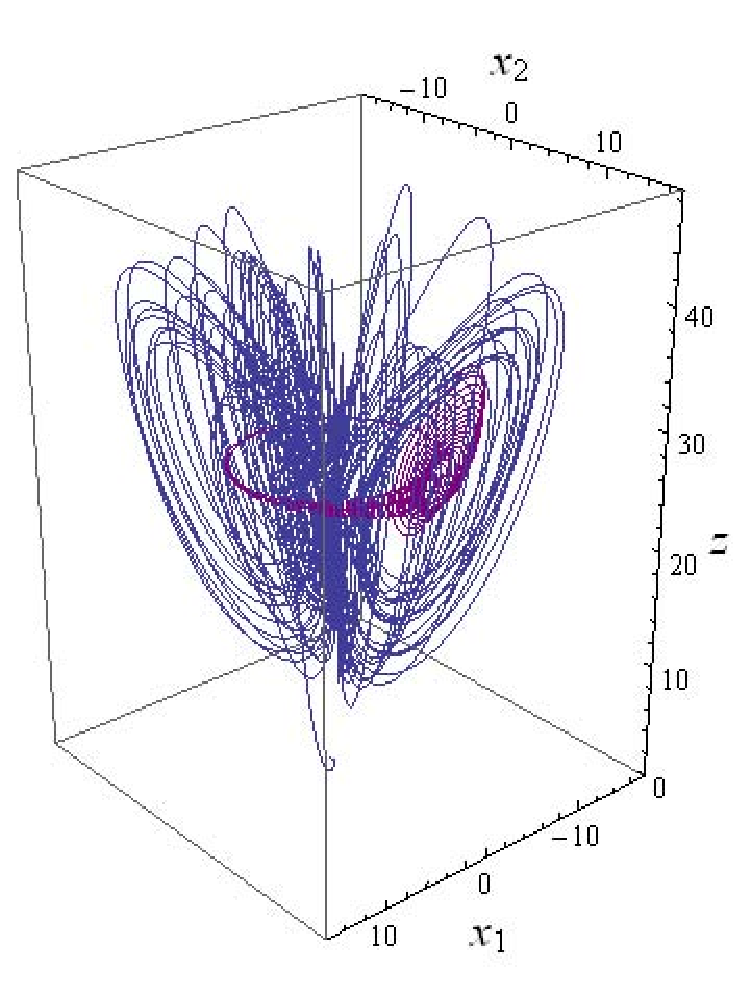
\includegraphics[width=0.35\textwidth]{CLEx1x2zRelEqu}
\end{center}
\caption{
Cartesian $\{x_1,x_2,z\}$ plot of the \cLf\ (a) with initial point
close to $\REQB{1}$, (b) superimposed over the strange attractor of
\reffig{fig:CLEx1x2z}.
    }
\label{fig:CLERelEqui}
\end{figure}
%%%%%%%%%%%%%%%%%%%%%%%%%%%%%%%%%%%%%%%%%%%%%%%%%%%%%%%

From
here on, we examine the properties of the point defined
above as $\ssp_{\REQB{}1}$.

\subsection{\Rpo s}
\label{SF:rpos}

\paragraph{Definition:
           \Rpo}
$p$ is an orbit $\pS_p$ in {\statesp} $\pS$, a set of relative periodic
points exactly recur
    \toCB
\beq
\ssp (0) = \LieEl_p \ssp (\period{p} )
    \,,\qquad
\ssp (\tau) \in \pS_p
    \,,
\label{RPOrelper1}
\eeq
at a fixed {\em relative period} $\period{p}$, but
shifted by a fixed group action ${\LieEl_p}$
which brings the endpoint $\ssp (\period{p} ) $
back into the initial point $\ssp (0) $.
The group action ${\LieEl_p}=\LieEl(\gSpace_p)$ parameters  \toCB
$\gSpace = (\gSpace_1,\gSpace_2,\cdots\gSpace_N)$
are referred to as ``phases,'' or ``shifts.''
%
In general these phase are irrational, and the trajectory  \toCB
sweeps out ergodically the group orbit without ever closing
into a \po.

In presence of a continuous symmetry we define the
\emph{{\FloquetM} for a \rpo} as the {\jacobianM} evaluated
at the period $\period{p}$ and rotated back into a \po\ by the
group action $\LieEl(\gSpace_p)$:
    \toCB
\beq
 \jMps_p(\ssp) = \LieEl(\gSpace_p)\jMps^\period{p}(\ssp)
    \,,\qquad
\ssp  \in \pS_p
\,.
\ee{SF:symPrimJac}
The argument of \refsect{sect:SFpos} goes through also in
the presence of a group rotation,
and \refeq{SF:transpEigPO} is correct for \rpo s as well.

\subsection{Marginal eigenvalues}

The {\jacobianM} of a periodic orbit has marginal eigenvalues
when there is either a continuous symmetry (which can use to
reduce the problem) or a non-hyperbolicity in the flow (which
is not as easy to deal with).

To see that each continuous symmetry has a corresponding
marginal eigendirection, let $\ssp$ be any point on a periodic
orbit p with period $\period{p}$. If $\LieEl$ is any element in
the continuous symmetry Lie group $\Group$, then $f^t(\LieEl \ssp)
= \LieEl f^t(\ssp)$. By definiton, $\jMps^t(\ssp)
\delta \ssp = \delta f^t(\ssp)$.
Close to identity $\LieEl = 1+\delta
\theta \cdot \Lg$ is an infinitesimal Lie group element and
$\delta \ssp = \ssp - \LieEl \ssp = \ssp - (1+\delta \theta
\cdot \Lg) \ssp  = \delta \theta \cdot \Lg \ssp,$
so
$\delta f^{\period{p}}(\ssp) = f^{\period{p}}(\ssp) -
f^{\period{p}}(\LieEl \ssp)= f^{\period{p}}(\ssp) - \LieEl f^{\period{p}}(\ssp) =
\ssp - \LieEl \ssp = \delta \theta \cdot \Lg \ssp$.
This gives us
$\jMps_p(\ssp) \delta \theta \cdot \Lg \ssp = \delta
\theta \cdot \Lg \ssp$,
\ie, a set of marginal direction eigenvectors
\beq
 \jMps_p(\ssp) \groupTan_{a}(\ssp) =
\groupTan_{a}(\ssp)
\ee{SF:symMargEig}
with unit eigenvalues $\ExpaEig_a=1$,
where $\groupTan_{a}(\ssp)$ is a group tangent \refeq{PC:groupTan}.
    \PC{prove this for a \rpo, using definition \refeq{SF:symPrimJac};
        the \po\ marginal eigenvalue should be a special case.}


\subsection{Stability of \reqva\ in \reducedsp}
%SF June 22 2010

Using the parameters \refeq{SiminosPrmts}, we get the
 $\REQB{1}$ stability eigenvalues
\[
0.0938 \pm 10.1945i,-22.0000,-13.8534,-11.009
\]
with corresponding eigenvectors
        \PC{ChaosBook convention is to order eigenvalues
        from most positive (unstable) to the most negative.
        \\
        Replace complex eigenvectors by the real,
        imaginary parts, as that is what you actually use - I
        did this in \refeq{eigVecQ1}.
        }
\bea
&&(0.3378\mp 0.3411i,0.6887,0.0017\mp 0.0031i,0.5133\mp 0.1706i,-0.0029\mp 0.0511i)
\continue
&&(0.9939,0.0470,0.0009,-0.0994,0.0051)
\continue
&&(-0.8966,0.3457,0.0097,-0.2755,0.0246)
\continue
&&(0.0210,-0.0203,-0.995,0.0095,-0.0011)
\nnu
\eea
These are the same as the eigenvalues found using polar coordinates with the addition of $-22.0000$.
    \PC{
    ``the addition of $-22.0000$'' means what?
    }

The equations of motion for trajectory kept in a hyperplane by rotation under the symmetry group are:
\bea
    \dot{\gSpace}_a (\sspRed) &=&
    \frac{\dotProd{v(\sspRed)}{\sliceTan{a}}}
         {\dotProd{\groupTan(\sspRed)}{\sliceTan{}}}
    \continue
    u(\sspRed) &=& v(\sspRed)-\dot{\gSpace}(\sspRed)  \cdot \groupTan(\sspRed)
\eea
where $v(\sspRed)$ is the velocity of the full \statesp\ flow, $\groupTan(\sspRed)$ is the tangent to the group action, and $\sliceTan{}$ is the vector normal to the hyperplane of the slice. Using this equation we get that the {\stabmat} $\MvarRed$ for the system in \reducedsp\ is given by:
    \PC{Stefan's version was
\[
M_{ij} =
A_{ij}-c I_{ij} -(Tx)_i\,(\frac{\frac{\partial v}{\partial x_i}\cdot \sliceTan{}}
        {Tx \cdot \sliceTan{}}
      - c \frac{\frac{\partial (Tx)}{\partial x_j}\cdot \sliceTan{}}{Tx \cdot \sliceTan{}})
\]
    hopefully no errors introduced in my rewrite
    }
\beq
{\MvarRed}(\sspRed)_{ij} = \Mvar(\sspRed)_{ij}-\velRel \cdot \Lg_{ij}
     -\groupTan(\sspRed)_i\,\left(
     \frac{\frac{\partial v}
     {\partial x_j}\cdot \sspRed}{\dotProd{\groupTan(\sspRed)}{\sliceTan{}}}
     - \velRel \frac{\frac{\partial (\groupTan(\sspRed))}
              {\partial x_j}\cdot \sliceTan{}
              }{\dotProd{\groupTan(\sspRed)}{\sliceTan{}}}
              \right)
\ee{SF:redJacob1}

                                                    \exerbox{exer:Reducedstab}

\subsection{Eigen-system of the slice \stabmat}

As in \refsect{sect:stability}, we now find and plot the
eigen-system of the \stabmat\ in order to understand the
stability of $\REQB{1}$.
Rebecca finds the eigenvalues
\beq
(\lambda_{1,2},\lambda_3,\lambda_4)
= (0.0938179 \pm 10.1945 i,-11.0009,-13.8534)
\ee{RW:REQB1eigvals}
with the eigenvectors
\bea
\Re e_{1} &=& \Re e_{2} = (-0.266121, -0.0321133, 0.00034139, 0.719222)
\continue
\Im e_{1}  &=& -\Im e_{2} = (-0.295017, 0.569063, -0.000551886,0)
\continue
e_3 &=& (-0.0883591, -0.0851485, -0.989135, -0.0809553)
\continue
e_4 &=& (-0.855586, -0.329912, -0.00273531, -0.398902)
\,.
\label{eigVecQ1}
\eea

As in \refsect{sect:stability}, we can also plot the flow
with an initial point very near to
$\REQB{1}$ along one of the eigenvectors.
% \refFig{fig:CLEQ1} shows just this.
                                                    \exerbox{exer:EigenQ1}
                                                    \exerbox{exer:PlotPolEigenQ1}

\subsection{\Rpo\ stability in \reducedsp}

    \PC{Stefan, please write up your ``three programs for approximating the \jacobianM\ along any trajectory.'' Derive here \rpo\ {\monodromyM} in the \reducedsp, test it on some of the Evangelos \rpo s for \cLe.
    }

\section{Newton searches for \po s}

We have already seen how knowing periodic orbits and their
stability can help us to understand the dynamics of the
system, but there still is the question of how to actually
find periodic orbits.

Suppose we are trying to find the periodic orbits of a
system. This means we want to find $x$ and $T$ such that $\ssp =
f^T\left(\ssp\right)$,
% $\Rightarrow 0 = \ssp-f^T\left(\ssp\right)$
where $f^T$ is the trajectory at
time $T$. We shall use Newton's method to search zeros of the function
$F\left(\ssp,T\right) = \ssp - f^T\left(\ssp\right)$. Let
$\left(\ssp,T\right)$ be an initial guess for Newton's method
close to an actual solution $\left(\ssp + \Delta x,T + \Delta
T\right)$, \ie\ $0 = \ssp +\Delta \ssp - f^{T+\Delta
T}\left(\ssp + \Delta \ssp\right)$. Keeping the Taylor series
to linear order
\[
0 \approx \ssp-
f^T\left(\ssp\right) + \left(I -
\jMps\left(\ssp\right)\right)\Delta \ssp -
v\left(f^T(\ssp)\right)\Delta T
\]
we get the Newton iteration estimate for
$(\Delta \ssp,\Delta T)$

We already know that if $\ssp$ is on a periodic orbit then
$
% \jMps\left(\ssp\right) v(\ssp) = v\left(\ssp\right) \Rightarrow
\left(I-\jMps\left(\ssp\right)\right) v\left(\ssp\right) =
0$, so $I-\jMps\left(\ssp\right)$ becomes
non-invertible as $\ssp$ approaches a periodic orbit.
%$\left(I-\jMps\left(\ssp\right)\right) v\left(\ssp\right)\approx 0$.
If $\Delta x$ is in the direction of
$v\left(\ssp\right)$ then
$\left(I-\jMps\left(\ssp\right)\right) \Delta \ssp \approx 0$
so the equation becomes very costly to solve accurately. This
means that we need to constrain the $\Delta \ssp$ to be
transverse to the flow during a Newton's iteration. We do this
by requiring $\Delta x$ satisfy
\beq
v (\ssp)^T \Delta \ssp = 0
\,.
\ee{SF:NewtonTransv}
We then get the system
\beq
    \begin{pmatrix}
        I-\jMps(\ssp)& \partial v(\ssp)\\
        v(\ssp)& 0
    \end{pmatrix}
    \begin{pmatrix}
        \Delta \ssp\\
        \Delta t
    \end{pmatrix}
    =-
    \begin{pmatrix}
        \ssp - f(\ssp)\\
        0
    \end{pmatrix}
\eeq
This problem was caused by the velocity vector being an
eigenvector of the {\jacobianM} with unit Floquet
multiplier. Thus for every unit Floquet multiplier we
need to add a constraint. It was
already shown that for every dimension of a continuous
symmetry there is a unit Floquet multiplier. For each of
these we need to add a constraint
similar to \refeq{SF:NewtonTransv}.

Next consider the same situation, but instead we will use a
cost (or error) function $I\left(\Delta \ssp\right) =
\left(\ssp + \Delta \ssp - f\left(\ssp + \Delta
\ssp\right)\right)^2/2$. If $\ssp+\Delta \ssp$ is on a
periodic orbit then $I\left(\delta \ssp\right)$ and its
linear in $\Delta x$ approximation  $\left(\ssp + \Delta \ssp
- f\left(\ssp+ \delta
\ssp\right)\right)\left(I-\jMps\left(\ssp\right)\right)$ are
both equal to 0. This cost function measures how
far the point $\ssp+ \Delta \ssp$ is from being a zero of the
function $F(\ssp, \Delta \ssp) = \ssp - f(\ssp)$. The cost
function gives a non-negative value, and its zeros are the
points on periodic orbits, so if we can find a way to
minimize the function then we would either find a periodic
orbit or learn that there are not any near our initial guess
(if the local minimum is not zero then there is no zero
nearby).

The linear approximation of the cost function is zero at a
periodic orbit, so the cost function is dominated by the
second order term near the orbits. Expanding $I(\Delta \ssp)$
to the second order, we get that $I \approx \tilde{\Delta
\ssp}^2/2 + (\ssp - f(\ssp)) \tilde{\Delta \ssp} +
(\ssp-f(\ssp))^2/2$ where $\tilde{\Delta \ssp} =
(I-\jMps(\ssp))\Delta \ssp$.

\section{Hilbert polynomials}
\label{SF:relStab}

The polynomials \refeq{eq:ipLaser} form a Hilbert basis for the \cLe.
\beq
\begin{split}
    u_1 &= x_1^2+x_2^2 \cont
    u_2 &= y_1^2+y_2^2 \cont
    u_3 &= x_1 y_2-x_2 y_1\cont
    u_4 &= x_1 y_1+x_2 y_2\cont
    u_5 &= z\,.
    \label{eq:ipLaser}
\end{split}
\eeq
In terms of the polar coordinates for the \cLe, these polynomials are
	\PC{shouldn't the first two be $\rho_1^2,\rho_2^2 $?}
\beq
\begin{split}
    u_1 &= \rho_1 \cont
    u_2 &= \rho_2 \cont
    u_3 &= - \rho_1 \rho_2 \sin \theta \cont
    u_4 &= \rho_1 \rho_2 \cos \theta \cont
    u_5 &= z\,.
    \label{eq:hilPolar}
\end{split}
\eeq
The \cLe\ in the Hilbert basis are:
\beq
\begin{split}
  \dot{u}_1 &=2\,\sigma\,(u_4-u_1)\,,\\
  \dot{u}_2 &=-2(\,u_2 - r_2\, u_3 -\,(r_1-u_5)\,u_4)\,,\\
  \dot{u}_3 &=-(\sigma\, +1)\,u_3+r_2\, u_1+e\, u_4\,,\\
  \dot{u}_4 &=-(\sigma\, +1)\,u_4+\,(r_1-u_5)\,u_1+\sigma\, u_2-e\,u_3\,,\\
  \dot{u}_5 &=u_4-b\, u_5\,.
\end{split}
\label{eq:CLEip}
\eeq
The {\reqv} in polar coordinates is
\[
( \rho_1 , \rho_2 , \theta , z ) = (\sqrt{b (r_1 -d)},\sqrt{b d (r_1 -d)},\theta_Q, r_1 -d)
\]
where $d = 1+ \frac{e^2}{(\sigma +1 )^2}$ and $\theta_Q$ is the angle such that
\[
\cos \theta_Q = \sqrt \frac{1}{d}
    \,,\qquad
\sin \theta_Q = -\sqrt \frac{d-1}{d}
\,.
\]

\exercise{Hilbert basis singularities}{\label{exer:CLEipSyz}
% Predrag extracted from siminos/blog/CLEflotsam      Jun  5 2010
% also ChaosBook \example{Hilbert basis singularities}{\label{exam:CLEipSyz}
%
When one takes syzygies into account in rewriting a
dynamical system, singularities are introduced. For instance,
eliminate $u_2$ using the syzygy, and show that you get
the reduced set of equations,
	\PC{I removed
$  \dot{u}_2 = -2\left(\,\frac{u_3^2+u_4^2}{u_1} - \rho_2\, u_3
                -\,(\rho_1-u_5)\,u_4\right)
$
            }
\bea
  \dot{u}_1 &=& 2\,\sigma\,(u_4-u_1)
                \continue
  \dot{u}_3 &=& -(\sigma\, +1)\,u_3+\rho_2\, u_1+e\, u_4
                \continue
  \dot{u}_4 &=& -(\sigma\, +1)\,u_4+\,(\rho_1-u_5)\,u_1
                +\sigma\, {(u_3^2+u_4^2)}/{u_1}-e\,u_3
                \continue
  \dot{u}_5 &=& u_4-b\, u_5
\,,
\label{eq:CLEipSyz}
\eea
singular as $u_1\rightarrow 0$. (PC: check this - there might
be errors)
\authorES{}
    } %end \exer{Hilbert basis singularities}

The {\stabmat} in the Hilbert basis for the \cLe\ is
	\PC{This is [5$\times$5], but there are only 4 independent
            variables. How does that show up in the eigensystem of
	    {\stabmat}?}
\beq
\begin{split}
\mathbb{A}=
\left(
\begin{array}{ccccc}
-2 \sigma & 0 & 0 & 2 \sigma & 0\\
0 & -2 & 2 r_2 & 2 (r_1 - u_5) & -2 u_4\\
r_2 & 0 & -(\sigma +1 ) & e & 0\\
(r_1 -u_5 ) & \sigma & -e & -(\sigma +1 ) & -u_1\\
0 & 0 & 0 & 1 & -b
\end{array}
\right)
\end{split}
\eeq

\section{Raw \slice s}
\label{sect:raw}
    \PC{this is temporary, until \refsect{sect:slices} is finalized.
        Stefan, please compare the formulas in the two, in order to
        improve your \LaTeX\ arts, then remove this section.}

Our goal is to show that if we choose the slice to be the hyperplane normal to the group tangents at a point, then this slice intersects all group orbits.

For this proof we will assume that the Lie group is compact and connected (so we can represent any group element by $\LieEl=e^{\gSpace \cdot \Lg}$ where $\gSpace \cdot \Lg=\sum \gSpace_a \Lg_a$).\\
\\
\noindent Fix $\ssp' \in \pS$.\\
We will be looking at the hyperplane $\bar{\pS}$ that is normal to all the group rotation tangents at $\ssp'$, \ie\ all points $\ssp$ with $<\ssp|\groupTan_a(\ssp')>=0$ (where $\groupTan_a(\ssp')=\Lg_a \ssp'$ are the group tangents at $\ssp'$).\\
\\
Let $\ssp \in \pS$ be any point in the phase space.\\
We want to show that there is a point on the group orbit of $\ssp$ which lies in $\bar{\pS}$, \ie\ there is a group element $\LieEl=e^{\gSpace \cdot \Lg}$ such that $<\LieEl \ssp|\groupTan_a(\ssp')>=0$ for all $a$.\\
\\
To show this we will look at the function $f_{\ssp}(\gSpace)=<\ssp'|e^{\gSpace \cdot \Lg} \ssp>$.\\
$f_{\ssp}$ is a continuous and differentiable function by how it was defined ($e^{\gSpace \cdot \Lg}$ is both continuous and differentiable and $f_{\ssp}$ is just the inner product of this with a constant, so it is also continuous and differentiable).\\
This tells us that if $\gSpace_E$ is an extremum of $f_{\ssp}$ then all of the first order partial derivatives of $f_{\ssp}$ will be zero at $\gSpace_E$ since $f_{\ssp}$ is differentiable.\\
This would mean $\frac{\partial f_{\ssp}(\gSpace_E)}{\partial \gSpace_a}=0$, so $<\ssp'|\Lg_a e^{\gSpace_E \cdot \Lg} \ssp>=0$.\\
$\Lg_a$ is anti-hermitian, so $0=<\ssp'|\Lg_a e^{\gSpace_E \cdot \Lg} \ssp>=<-\Lg_a \ssp'|e^{\gSpace_E \cdot \Lg} \ssp>=-<\Lg_a \ssp'|e^{\gSpace_E \cdot \Lg} \ssp>$ giving us that $<\groupTan_a(\ssp')|e^{\gSpace_E \cdot \Lg} \ssp>=0$.\\
We therefore have that $e^{\gSpace_E \cdot \Lg} \ssp$ is normal to all the group tangents of $\ssp$ so it is in $\bar{\pS}$.\\
This means that any extrema of $f_{\ssp}$ are in the slice.\\
All that is left to do then is to show that $f_{\ssp}$ has extrema.\\
\\
Define $h(y)=<\ssp'|y>$.\\
$h$ is continuous it is the inner products with a constant.\\
Next consider $h$ on $\pS_{\ssp}$ (the group orbit of $\ssp$).\\
$\pS_{\ssp}$ is compact since we are working with a compact Lie group.\\
$h$ is continuous and $\pS_{\ssp}$ is compact, so $h$ achieves its extrema on $\pS_{\ssp}$, or more specifically its minimum, \ie\ there is a point $y_{min} \in \pS_{\ssp}$ such that $h(y)\geq h(y_{min})$ for all $y\in \pS_{\ssp}$. $y_{min} \in \pS_{\ssp}$ means that $y_{min}=e^{\gSpace_{min} \cdot \Lg} \ssp$ for some $\gSpace_{min}$.\\
\\
For any $\gSpace$, $f_{\ssp}(\gSpace)=<\ssp'|e^{\gSpace \cdot \Lg} \ssp>=h(e^{\gSpace \cdot \Lg} \ssp)$. We also know that $e^{\gSpace \cdot \Lg} \ssp \in \pS_{\ssp}$ by the definition of group orbit, so $f_{\ssp}(\gSpace)\geq h(y_{min})$ for all $\gSpace$. We have that $y_{min}=e^{\gSpace_{min} \cdot \Lg} \ssp$, so $h(y_{min})=f_{\ssp}(\gSpace_{min})$.
This means $\gSpace_{min}$ is such that $f_{\ssp}(\gSpace)\geq f_{\ssp}(\gSpace_{min})$ for all $\gSpace$, so it is a minimum of $f_{\ssp}$.\\
Therefore, $e^{\gSpace_{min}\cdot \Lg} \ssp$ is in $\bar{\pS}$, so there is a point on the group orbit of $\ssp$ that is in the slice.\\


\section{Conclusions}

Both the {\mslices} (or the \mframes) integration within the
\slice\ are still under development.\PC{to Stefan: keep
editing this every so often}

Future work should investigate in more depth [...].
New methods [...] In this project I have discussed, understood,
and tested [...] as applied to \cLe\.
Much work still remains before these are viable
methods for higher-dimensional flows.

